\chapter{Functional Flow Diagram}\label{chap:baseline_ffd}
To gain insight in the system that is to be designed, a \acrlong{ffd} is generated. This \acrshort{ffd} presents the high level functions that the system should be able to perform, in chronological order. These functions are presented in the flow diagram of \cref{fig:basline_ffd}. 

\begin{figure}[H]
    \centering
    %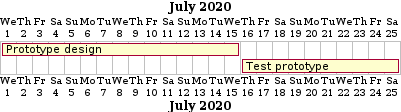
\includegraphics[width=0.6\linewidth]{Images/Diagrams/trivial_gantt.png}
    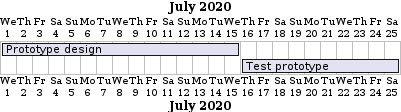
\includegraphics[width=0.6\linewidth]{latex/project8/Images/Diagrams/trivial_gantt.png}
    \caption{A functional flow diagram with the high-level functions of the system that is to be designed.}
    \label{fig:baseline_ffd}
\end{figure}

\begin{enumerate}
    \item Initialise \& start space-related function on neuromorphic architecture without brain adaptation implementation.
    \item Initialise \& start space-related function on neuromorphic architecture with brain adaptation implementation.
    \item Endure modelled space radiation on neuromorphic architecture.
    \item Measure space-related function performance without brain adaptation implementation.
    \item Measure space-related function performance with brain adaptation implementation.
    \item Report any performance difference between with- and without brain adaptation.
    \item Determine significance of difference.
\end{enumerate}

From these high level functions, a more detailed functional breakdown diagram is generated.

\section{Detailed Functional Flow Diagram}\label{sec:baseline_detailed_ffd}
\begin{enumerate}
    \item Initialise \& start space-related function on neuromorphic architecture without brain adaptation implementation.    
    \begin{enumerate}
        \item Boot/initialise neuromorphic architecture
        \item Load function.
        \item Load function data.
    \end{enumerate}
    \item Initialise \& start space-related function on neuromorphic architecture with brain adaptation implementation.
    \begin{enumerate}
        \item Boot/initialise neuromorphic architecture
        \item Load brain adaptation.
        \item Load space-related function.
        \item Load space-related function data.
    \end{enumerate}
    \item Render and endure modelled space radiation on neuromorphic architecture.
    \begin{enumerate}
        \item Determine simulated space radiation pattern of neuromorphic space architecture.
        \item Expose neuromorphic architecture to simulated space radiation pattern.
        \item Complete space-related function.
        \item Return results of space-related performance.
    \end{enumerate}
    \item Measure space-related function performance without brain adaptation implementation.
    \begin{enumerate}
        \item Retrieve space-related function output.
        \item Convert space-related function output to score.
    \end{enumerate}
    \item Measure space-related function performance with brain adaptation implementation.
    \item \begin{enumerate}
        \item Retrieve space-related function output.
        \item Convert space-related function output to score.
    \end{enumerate}
    \item Report difference between the scores of the architectures with- and without brain adaptation.
    \item Determine significance of difference.
\end{enumerate}

\subsection{Description}\label{subsec:description}
\begin{enumerate}
    \item Initialise \& start space-related function on neuromorphic architecture without brain adaptation implementation.
    \begin{itemize}
        \item To run a function on the neuromorphic architecture, it will have to be booted and initialised. The function that will be ran on the neuromorphic architecture is space related, to increase the level of representativeness of this study, in terms of space applications. The initalisation allows for loading the space related function that is to be executed. Additionally, the space related function may require (training) data on which it is ran. For example, a Martian rover that has a function that identifies rocks in its environment, may be partially simulated by loading a (labelled) dataset of Martian images.

        To run the function without brain adaptation implementation, allows for the creation of a baseline to which the brain adaptation performance can be compared.
    \end{itemize}
    \item Initialise \& start space-related function on neuromorphic architecture with brain adaptation implementation.
    \begin{itemize}
        \item The intialisation of the brain adaptation implementation can occur, before, during or after the loading of the space related function. Which of these options is selected depends on the more detailed design process.
    \end{itemize}
    \item Endure modelled space radiation on neuromorphic architecture.
    \begin{itemize}
        \item The radiation robustness of the neuromorphic architecture can be tested by exposing the neuromorphic architecture to the radiation that it would experience in a space application. To determine what this radiation is, a relevant space mission and space function are selected. The time, position and orientation of the spacecraft in such a mission is then used to derive the radiation pattern to which the radiation may be exposed. This radiation is pattern is then used to determine to which (simulated) radiation the neuromorphic architecture will be exposed.
    \end{itemize}
    \item Measure space-related function performance without brain adaptation implementation.
    \begin{itemize}
        \item The performance of the space related function without brain adaptation implementaiton on the neuromorphic architecture is measured before, during and/or after radiation exposure. Which of these measuring moments are used, is still to be determined by the detailed design process. This measurement then serves as a comparison baseline to put the impact of the brain adaptation implementation into context.
    \end{itemize}
    \item Measure space-related function performance with brain adaptation implementation.
    \item \begin{itemize}
        \item Once a baseline for comparison is established, the space related function can be ran again on the neuromorphic hardware, whilst being exposed to radiation. In this second setting, the brain adaptation implementation is used in an attempt to increase the radiation robustness of the neuromorphic architecture. The performance of the space related function is then measured before, during and/or after radiation exposure. Which of these measuring moments are used, is still to be determined by the detailed design process. 
    \end{itemize}
    \item Report any performance difference between with- and without brain adaptation.
    \item \begin{itemize}
        \item If any performance difference is observed between the space related function with- and without brain adaptation implementation, it will be computed and stored.
    \end{itemize}
    \item Determine significance of difference.
    \item \begin{itemize}
        \item An analysis is performed to determine the level of significance  of any observed difference.
    \end{itemize}
\end{enumerate}